\documentclass[11pt]{article}
\usepackage[a4paper,margin=24mm]{geometry}
\usepackage[T1]{fontenc}
\usepackage{amsmath,amsthm,newtxtext,newtxmath,microtype}
\usepackage{booktabs,tabularx,array,graphicx,xcolor}
\usepackage{algorithm,algpseudocode,enumitem}
\usepackage{float}
\usepackage{tikz}
\usetikzlibrary{positioning,arrows.meta,fit}
\usepackage[font=small,labelfont=bf]{caption}
\usepackage[hidelinks]{hyperref}
% Allow URLs to break at any character (avoids underfull boxes in the bibliography).
\makeatletter
\def\UrlBreaks{\do\.\do\@\do\\\\\do\/\do\_\do\|\do\-\do\+\do\=\do\#\do\$\do\%\do\^\do\&\do\*\do\~\do\a\do\b\do\c\do\d\do\e\do\f\do\g\do\h\do\i\do\j\do\k\do\l\do\m\do\n\do\o\do\p\do\q\do\r\do\s\do\t\do\u\do\v\do\w\do\x\do\y\do\z\do\A\do\B\do\C\do\D\do\E\do\F\do\G\do\H\do\I\do\J\do\K\do\L\do\M\do\N\do\O\do\P\do\Q\do\R\do\S\do\T\do\U\do\V\do\W\do\X\do\Y\do\Z}
\makeatother
\usepackage{fancyhdr}
\pagestyle{fancy}\fancyhf{}\fancyhead[L]{\small Adaptive HACT}\fancyhead[R]{\small Manuscript revision 5.1}\fancyfoot[C]{\thepage}
\setlength{\headheight}{14pt}\setlength{\parskip}{3pt}\setlength{\emergencystretch}{2em}
\newtheorem{theorem}{Theorem}\newtheorem{proposition}[theorem]{Proposition}\newtheorem{lemma}[theorem]{Lemma}
\theoremstyle{definition}\newtheorem{definition}[theorem]{Definition}
\newcommand{\PASS}{\mathsf{PASS}}\newcommand{\FAIL}{\mathsf{FAIL}}\newcommand{\UNKNOWN}{\mathsf{UNKNOWN}}
\newcommand{\E}{\mathbb E}\newcommand{\Prb}{\mathbb P}\newcommand{\ind}{\mathbf 1}\newcommand{\R}{\mathcal R}
\DeclareMathOperator*{\argmin}{arg\,min}
\hypersetup{pdftitle={Adaptive HACT: Hyperedge-Aware, Identity-Stable Verification Evidence for Agentic Systems},pdfauthor={Research manuscript; author information pending confirmation}}
\title{\vspace{-9mm}\textbf{Adaptive HACT: Hyperedge-Aware, Identity-Stable Verification Evidence for Agentic Systems}}
\author{Research manuscript\thanks{Author names and affiliations require confirmation before submission. Mathematical development, implementation, experiments, and writing were AI-assisted.}}
\date{October 4, 2026 \quad | \quad Manuscript revision 5.1 \quad | \quad Artifact 5.0}
\begin{document}
\maketitle
\begin{abstract}
Agentic software pipelines increasingly gate candidate changes on suites of tests, analyses, and policy checks, but the evidence supporting a commit decision can be much larger than the final verdict. Adaptive HACT asks whether that evidence can be reorganized for cheaper diagnostic delivery without changing the acceptance contract. The central abstraction is \emph{evidence-layout independence}: stable check identities and candidate/checker/environment bindings define semantics, while a separate layout plane only aggregates trusted completion records. Generation fencing makes authorization invariant to valid layout permutations and migrations. Because packet work depends on which \emph{sets} of checks become final together, we score recorded completion hyperedges rather than treat pairwise affinity as the cost model. The practical compiler uses a learned order with a compact balanced eight-ary tree; exact alphabetic dynamic programming is retained as a fixed-order reference. In 27 frozen train/validation/held-out workloads, clustered completions reduce held-out padded evidence by 23.43\%, 10.75\%, and 5.56\% at 128, 512, and 1,024 checks, with positive reductions in all nine clustered seeds; independent and global controls show essentially no benefit. Re-aggregating twelve archived source candidates reduces whole-epoch compressed bytes by 4.36--41.84\% versus original-order fixed8, while exact layouts remain 1.52--11.68\% smaller than the practical layout. Root-status text is identical across all twelve layout triples. A service-matched break-even model separates representation savings from the cost of adopting verification. The measured claim is therefore narrow: HACT reduces hierarchical verification-evidence cost when completion structure exists, while preserving the declared acceptance semantics; live-model quality, physical-WAN speedup, and provider token billing are outside the present evidence.
\end{abstract}
\noindent\textbf{Keywords:} agentic systems; verification evidence; completion hyperedges; evidence-layout independence; bounded diagnostics; cost-aware layout selection.

\section{Introduction}
Autonomous and multi-agent software systems can generate many candidate actions in parallel, but accepting a candidate is a different problem from generating it. A deployment gate may need evidence from tests, static analyzers, policy checks, environment probes, and integration checks. The final decision may be one bit, yet debugging, audit, and remote supervision can require a much larger transcript of intermediate evidence. That creates a representation problem: reorganizing the transcript may save bytes and retrieval work, but it must never change which checks are required or turn missing evidence into a pass.

Adaptive HACT treats verification semantics and evidence representation as separate planes. The semantic plane binds a candidate to a registry of stable check identities and to the checker and environment that produced each result. The layout plane is free to permute those identities and aggregate their records into bounded packets. This separation creates a useful systems invariant: layout learning can change \emph{where evidence is stored and how much is emitted}, but not \emph{what must be true before authorization}.

\begin{figure}[t]
\centering
\resizebox{\linewidth}{!}{%
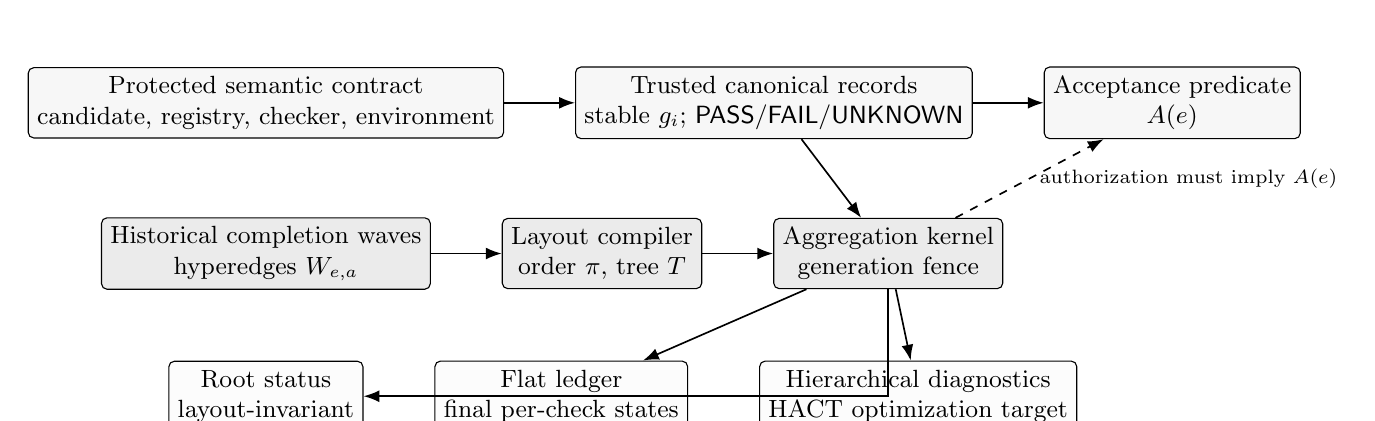
\begin{tikzpicture}[
  >=Latex,
  box/.style={draw,rounded corners=2pt,align=center,minimum height=8mm,inner sep=3.2pt,font=\small},
  sem/.style={box,fill=black!3},
  lay/.style={box,fill=black!8},
  svc/.style={box,fill=black!1},
  arr/.style={->,line width=.6pt},
  node distance=7mm and 9mm]
  \node[sem] (contract) {Protected semantic contract\\candidate, registry, checker, environment};
  \node[sem,right=of contract] (records) {Trusted canonical records\\stable $g_i$; $\PASS/\FAIL/\UNKNOWN$};
  \node[sem,right=of records] (accept) {Acceptance predicate\\$A(e)$};
  \draw[arr] (contract) -- (records);
  \draw[arr] (records) -- (accept);

  \node[lay,below=10mm of contract] (history) {Historical completion waves\\hyperedges $W_{e,a}$};
  \node[lay,right=of history] (compiler) {Layout compiler\\order $\pi$, tree $T$};
  \node[lay,right=of compiler] (kernel) {Aggregation kernel\\generation fence};
  \draw[arr] (history) -- (compiler);
  \draw[arr] (compiler) -- (kernel);
  \draw[arr] (records) -- (kernel);
  \draw[arr,dashed] (kernel) -- node[right,font=\scriptsize]{authorization must imply $A(e)$} (accept);

  \node[svc,below=9mm of history] (root) {Root status\\layout-invariant};
  \node[svc,right=of root] (flat) {Flat ledger\\final per-check states};
  \node[svc,right=of flat] (diag) {Hierarchical diagnostics\\HACT optimization target};
  \draw[arr] (kernel) |- (root);
  \draw[arr] (kernel) -- (flat);
  \draw[arr] (kernel) -- (diag);
\end{tikzpicture}}
\caption{Adaptive HACT factors verification semantics from evidence representation. A valid layout may change aggregation cost and diagnostic hierarchy, but it cannot change the approved check set or the acceptance predicate. Root status and flat final ledgers are simpler services; HACT targets deployments that actually require hierarchical diagnostic evidence.}\label{fig:architecture}
\end{figure}

\paragraph{Evidence-layout independence.}
The paper formalizes the invariant sketched in Figure~\ref{fig:architecture}. A semantic registry and candidate identity are authoritative. Layouts are advisory data structures over those identities. A generation change invalidates layout-specific publication tickets and forces reconstruction from canonical trusted records. Under the stated trust assumptions, Theorem~\ref{thm:safety} shows that every authorized layout yields the same acceptance decision. This makes representation learning compatible with a fail-closed gate.

\paragraph{Why completion hyperedges matter.}
Evidence cost is driven by refresh events: when a set of checks becomes final, every ancestor packet intersecting that set may need to be re-emitted. Marginal activation rates lose joint structure, and pairwise co-activity can still miss the probability that a larger subtree is touched. We therefore treat each completion wave as a hyperedge and score candidate layouts on the observed sets directly. Pairwise affinity is used only to propose an order; it is not substituted for the actual full-wave objective.

\paragraph{Where HACT is useful.}
There are three distinct services. A consumer needing only a trusted final verdict should use a root-status projection. A consumer needing final per-check states can often use a flat ledger. HACT addresses the third case: a system that already needs bounded hierarchical evidence for diagnostics, audit, or constrained delivery. This service distinction prevents a common accounting error---crediting evidence compression with the unrelated cost of introducing a stricter verifier.

\paragraph{Contributions.}
The paper makes four claims, each tied to a concrete proof or experiment:
\begin{enumerate}[leftmargin=1.6em,itemsep=1pt,topsep=2pt]
\item \textbf{A semantic/representation factorization.} We define evidence-layout independence and give a generation-fenced implementation whose local authorization is invariant to valid permutations and migrations (Section~\ref{sec:model}; Theorem~\ref{thm:safety}).
\item \textbf{A hyperedge-sensitive cost model and compiler.} Full completion waves determine layout cost; Proposition~\ref{prop:pairwise} shows why pairwise affinity alone is insufficient. A practical no-DP compiler combines learned ordering with a balanced eight-ary tree, while exact alphabetic DP provides a fixed-order optimum for reference (Section~\ref{sec:compiler}).
\item \textbf{Migration- and service-aware operation.} Layout changes pay an explicit installation price, and deployment accounting compares codec-matched services instead of mixing bytes, tokens, and unrelated harness time (Sections~\ref{sec:online} and~\ref{sec:delivery}).
\item \textbf{Audited evidence with negative controls.} A frozen 27-workload study, 36 source-evidence replays, invariance checks, and independent arithmetic reconstruction identify both the structured regime where learning helps and the regimes where it does not (Section~\ref{sec:v5evaluation}).
\end{enumerate}
Clustering, balanced trees, alphabetic DP, compression, and break-even arithmetic are established ingredients. The contribution is their use under a verification-semantic invariant and a completion-hyperedge objective, together with evidence that distinguishes the useful regime from the null controls.

\paragraph{Scope.}
The experiments measure verification-evidence representation and local integration. They do not measure live-LLM coding quality, physical-WAN performance, or provider token billing. Those boundaries are collected in Section~\ref{sec:threats} instead of being repeatedly mixed into each positive result.

\paragraph{Roadmap.}
Section~\ref{sec:model} defines semantics and the cost model. Section~\ref{sec:compiler} develops the practical and exact-reference compilers; Section~\ref{sec:online} prices migration; Section~\ref{sec:safety} proves layout-independent local publication soundness. Sections~\ref{sec:implementation} and~\ref{sec:delivery} describe the implementation and service-matched accounting. Section~\ref{sec:v5evaluation} answers four evaluation questions, and Section~\ref{sec:conclusion} states the deployment implication.

\section{Related Work and Positioning}
\paragraph{Testing, impact analysis, and incremental computation.}
Test prioritization seeks earlier fault exposure~\cite{rothermel}; regression-test selection uses change dependencies~\cite{ekstazi,namerts}. The earlier IC-HACT ranker uses controlled mutation outcomes to prioritize checks, an instance of established fault-exposure methods. It is held fixed in the new source comparisons. Self-adjusting computation and build-system research already formalize dependency-aware recomputation~\cite{acar,build}. In contrast to test selection, our strict pass requires the entire approved registry on the identified candidate. We do not reproduce NameRTS or Ekstazi and claim no superiority over them.

\paragraph{Seriation and authenticated layouts.}
Spectral seriation orders items using an affinity matrix~\cite{atkins}. Average-linkage clustering likewise provides an established proximity-based ordering. Generalized alphabetic-tree optimization supplies the subtree/forest recurrence used here~\cite{alphabetic}. Workload-adaptive authenticated structures, including Huffman--Merkle Trees~\cite{hmt}, already optimize layouts under access patterns. Our price counts repeated completion-frontier updates, including strict-epoch construction, under a fixed packet cap. Pairwise affinity proposes an order; full hyperedge observations score it. No global optimality or unproved NP-hardness result is claimed for unrestricted joint ordering and tree synthesis.

\paragraph{Online decisions with switching costs.}
Fixed-share learning tracks changing experts~\cite{herbster}; dependent sampling reduces switches compared with independent weighted-majority draws~\cite{geulen}. Full-information and bandit switching-cost settings have different achievable regret guarantees~\cite{cesa}. We use the full-information setting because one recorded completion wave can be scored against every frozen certificate layout without reexecuting the tests. This is not full counterfactual feedback for arbitrary agent strategies: if a layout changes the tests' execution schedule or model behavior, our exogenous-cost assumption may fail. Our bound specializes established tools to measured layout-installation costs; it is not a new minimax online-learning result.

\paragraph{Agent runtime assurance and evaluation.}
Proof-Carrying Agent Actions~\cite{pcaa} and verification-portfolio commit gates~\cite{vpcontrol} address related action-governance problems. Our local certificates are neither signatures nor zero-knowledge proofs. SWE-bench evaluates real repository issues and patches~\cite{swebench}; our source mutations and scripted I/O repairs must not be called SWE-bench results. The current integration measures real orchestration and verification, not model reasoning quality.

\paragraph{Logging and serialization controls.}
Telemetry systems already batch and compress records~\cite{otel}. HACT is not a replacement for those techniques: fewer padded bytes need not imply fewer compressed bytes. We measure both. Moreover, flat result ledgers and a trusted root-status endpoint can be much smaller than an archive of all intermediate aggregation updates; they satisfy different delivery needs and must not be hidden from the comparison.

\section{Model and Trust Boundary}\label{sec:model}
\subsection{Semantic registry, execution, and display}
Let $\R=(g_0,\ldots,g_{n-1})$ be a nonempty approved registry of unique check IDs. The candidate identity is
\[
 e=(\mathrm{epoch},\mathrm{snapshot},\mathrm{checker},\mathrm{environment},\mathrm{registry}).
\]
The snapshot covers source and protected acceptance inputs. The checker and environment are explicitly bound; an epoch increases even after an ABA return to identical source bytes. Only a trusted runner submits final $\PASS$, $\FAIL$, or $\UNKNOWN$ records. Missing, stale, skipped, incompatible, or timed-out outcomes are not passes.

An execution permutation $\sigma_e$ determines when checks run. A layout $L=(\pi,T)$ independently maps tree positions to semantic registry indices. For a node covering positional interval $[i,j]$, its semantic coverage is
\begin{equation}
 G_L(i,j)=\{g_{\pi(i)},\ldots,g_{\pi(j)}\}.
\end{equation}
The stored layout must contain an exact permutation, and every internal node's children must partition its positional interval without gaps or overlaps. The task graph is outside this mathematical tree; one worker can discharge many checks, and one integration check can cover several workers.

The acceptance predicate is independent of both permutations:
\begin{equation}\label{eq:accept}
 A(e)=\ind\{\text{every }g_i\in\R\text{ has trusted, matching, current }\PASS\text{ evidence for }e\}.
\end{equation}
An observed fail permits rejection before all checks finish. It does not assert coverage of the unexecuted remainder. Acceptance is relative to the approved predicates, not proof of all program behavior.

\begin{definition}[Evidence-layout independence]\label{def:eli}
Fix a candidate identity $e$, semantic registry $\R$, and canonical trusted record set $E$. A verifier is \emph{evidence-layout independent} if valid layouts over the same registry may change representation cost, retrieval structure, and packet timing but cannot change the semantic projection of $E$, and no layout can authorize unless $A(e)$ holds.
\end{definition}
Definition~\ref{def:eli} is deliberately local to the declared verification contract. It does not claim that the contract itself is complete or that the checker is uncompromised; those are trust assumptions stated explicitly in Theorem~\ref{thm:safety}.

\subsection{Packet and lifecycle costs}
Each internal node of arity $d$ emits a fixed-width packet
\begin{equation}\label{eq:packet}
 c(d)=H+Sd,\qquad 2\le d\le b=\left\lfloor(C-H)/S\right\rfloor.
\end{equation}
Here $H=512$, $S=320$, and $C=3072$ bytes, so $b=8$. A mandatory field that exceeds its slot is rejected, not silently truncated. The cap applies to one certificate packet, not to all project memory, an entire registry manifest, or every LLM prompt. A manifest is a referenced control-plane artifact; its measured size is charged on migration.

Let $W_{e,1},\ldots,W_{e,q_e}$ be the semantic IDs whose final records become available between successive refreshes. For a strict new candidate epoch, the observed cost is
\begin{equation}\label{eq:strict}
 \ell_e(L)=W(L)+\sum_{a=1}^{q_e}\sum_{v\in\operatorname{int}(T)}
 c(d_v)\ind\{W_{e,a}\cap G_L(v)\ne\varnothing\},\quad
 W(L)=\sum_v c(d_v).
\end{equation}
The first term constructs the full initially unknown tree. The CLI batches an executed prefix into groups of eight, flushing its final partial group. A successful strict epoch runs the whole registry. This conservative implementation does not reuse a pass across distinct source snapshots.

We call each $W_{e,a}$ a \emph{completion hyperedge}: an arbitrary set of semantic obligations that becomes final between two refreshes. Equation~\eqref{eq:strict} consumes these sets directly through interval-hit events. Pairwise statistics may propose a permutation, but the scored objective remains higher-order.

We separately study persistent-state refresh traces that omit $W(L)$ at each tick, as in a cache with correctly specified incremental dependencies. Each topology installation is still cold and explicitly priced. These traces evaluate the controller's cost model; they are not the strict candidate-gate timing experiment. They do not demonstrate safe dependency inference from arbitrary code.

\subsection{Why more than invalidation or pairwise similarity is needed}
The inherited HACT result shows that marginal check activation cannot identify the best aggregation tree under joint invalidation (Appendix~\ref{app:separations}). IC-HACT further shows that even the full initial invalidation distribution cannot identify optimal progressive verification: early rejection and completion batching change the update sequence. Both distinctions remain relevant after allowing permutations.

\begin{proposition}[Pairwise affinity is insufficient for full-wave scoring]\label{prop:pairwise}
There exist two distributions with identical singleton and pairwise co-activity probabilities, hence identical Jaccard affinities, but different activation probabilities for the same three-check subtree.
\end{proposition}
\begin{proof}
On IDs $\{0,1,2\}$, let $P$ be uniform on $\emptyset,\{0,1\},\{0,2\},\{1,2\}$ and $Q$ uniform on $\{0\},\{1\},\{2\},\{0,1,2\}$. Every singleton has probability $1/2$, every pair has joint probability $1/4$, and its Jaccard affinity is $1/3$. Yet the probability that the triple is hit is $3/4$ under $P$ and $1$ under $Q$. Thus a packet emitted on that interval has different expected cost.\end{proof}
This elementary parity construction is not a new fact about higher-order statistics. Its implication for the compiler is specific: a pairwise clustering objective cannot substitute for scoring recorded completion hyperedges. It does not, by itself, prove that these two distributions have different globally optimal layouts.

\section{Learning Layouts Without Changing the Contract}\label{sec:compiler}
\subsection{Practical catalogue and full-wave selection}
Training waves define counts $N_i,N_{ij}$ and affinity
\begin{equation}
 a_{ij}=\frac{N_{ij}}{N_i+N_j-N_{ij}},
\end{equation}
with zero for an unobserved union and zero diagonal. The practical proposal uses established average-linkage clustering: join the closest current clusters, choose endpoint orientation by cross-boundary affinity, and break ties canonically. All semantic IDs, including disconnected and unseen checks, remain included exactly once.

Given the learned order, group consecutive leaves into blocks of at most eight, promote a singleton unchanged, and repeat upward. This bottom-up compact balanced construction does not call a tree optimizer. The catalogue retains the incumbent first, includes original-order fixed8 when distinct, and proposes learned-order fixed8. Identical layouts are deduplicated. A separate validation cohort scores complete completion waves, including initial construction; ties retain the incumbent. The API returns an advisory choice, not deployment authorization. The registry and packet cap cannot change during selection.

For any proposal $\pi$, training episodes supply interval weights
\begin{equation}\label{eq:weight}
 r_\pi(i,j)=1+\frac1m\sum_{e=1}^m\sum_a
 \ind\{W_{e,a}\cap G_L(i,j)\ne\varnothing\}.
\end{equation}
These weights also define the exact-DP reference below. Pairwise affinity \emph{proposes} an order; it does not replace the full-wave cost. The practical catalogue contains at most three candidates and uses no DP. Tree construction is $O(n)$ after ordering, not a linear-time claim for affinity construction, clustering or validation scoring. The reference implementation retains spectral ordering and exact fitting for research comparisons; neither is invoked by the practical default.

\subsection{Exact conditional tree synthesis}
Let $D(i,j)$ be the optimal subtree cost and $F_k(i,j)$ the optimal cost of an ordered forest with $k$ nonempty children. With infeasible states equal to $+\infty$,
\begin{align}
 D(i,i)&=0,\\
 F_1(i,j)&=D(i,j),\\
 F_k(i,j)&=\min_{i+k-2\le u<j}\{F_{k-1}(i,u)+D(u+1,j)\},\\
 D(i,j)&=\min_{2\le k\le\min(b,j-i+1)}\{r_\pi(i,j)c(k)+F_k(i,j)\}.\label{eq:dp}
\end{align}
\begin{theorem}[Exactness conditional on order]\label{thm:exact}
For a fixed $\pi$, nonnegative interval weights, and the packet model in Equation~\eqref{eq:packet}, Equation~\eqref{eq:dp} returns a minimizing feasible tree in $O(bn^3)$ time and $O(bn^2)$ space.
\end{theorem}
\begin{proof}
Every feasible root has an arity and a contiguous partition of its interval. Its local contribution depends only on that interval and arity; all remaining contributions belong to independent child subtrees. The forest recurrence enumerates every such partition. Induction on interval length proves exactness. There are $O(bn^2)$ states, each scanning at most $n$ splits. The apparent $F_1=D$ dependency is used only on shorter intervals when constructing a forest with at least two components.\end{proof}
This is a specialization of classical alphabetic-tree optimization~\cite{alphabetic}. The historical three-proposal reference multiplies compilation time by a constant, not by $n!$. Dense spectral computation can itself cost $O(n^3)$; the reference clustering implementation uses $O(n^2\log n)$ heap operations and $O(n^2)$ storage.

\begin{proposition}[Validation after learned ordering]\label{prop:validation}
Condition on a training set that fixes $K$ complete layouts. For $m$ independent identically distributed validation epochs with each layout cost in $[0,B]$, let $\widehat L$ minimize empirical validation cost. With probability at least $1-\delta$,
\begin{equation}
 J(\widehat L)\le\min_{L\in\mathcal C}J(L)+2B\sqrt{\frac{\log(2K/\delta)}{2m}}.
\end{equation}
\end{proposition}
\begin{proof}
Conditionally, the catalogue is fixed. Hoeffding's inequality~\cite{hoeffding} and a union bound over $K$ layouts bound every empirical mean error by the displayed radius without its factor two. Inserting empirical costs on either side of the empirical minimizer yields the result.\end{proof}
The guarantee is only relative to the fixed catalogue. It neither justifies choosing among learned permutations on their training errors alone nor covers distribution shift. We do not report this potentially loose bound as an empirical confidence interval; reported intervals use independent experimental seeds.

\subsection{Compiler identity and scope}
The practical default has no hidden microtree optimization. Exact DP is a reference and optional offline candidate. The block-backbone proposition and implementation remain in Appendix~\ref{sec:block} solely as an ablation; its restricted-class exactness does not override the observed simpler-baseline advantage. At 1,024 checks, order learning still takes seconds in our measurement, so layouts should be cached and compiled away from the agent's per-action path. Validation of padded costs does not optimize compressed archives or model tokenization; adoption must measure the actual delivery representation.

\section{Practical Online Selection: Price the Window, Not the Promise}\label{sec:online}
Freeze a compiled catalogue $\mathcal C=\{L_1,\ldots,L_K\}$. At event $t$, choose a layout before observing the current completion wave; afterwards score that same wave under every catalogue member. This is full-information feedback only because the check schedule is held fixed. It is not counterfactual feedback for arbitrary agent behavior.

A different layout is installed by serializing its canonical manifest and reconstructing its complete certificate tree:
\begin{equation}\label{eq:migration}
 M_{ij}=\begin{cases}0,&L_i=L_j,\\
 |\operatorname{manifest}(L_j)|+W(L_j),&L_i\ne L_j.
 \end{cases}\qquad
 \mathcal L_T=\sum_t\ell_t(A_t)+\sum_{t=2}^T M_{A_{t-1},A_t}.
\end{equation}
The initial installation is separate. These byte prices match the evaluated uncompressed migration protocol. A deployment using compression must measure its own priced wire representation; the DP objective is not automatically an optimum for a compressed log.

\paragraph{The primary practical rule.}
Let $\bar\ell_{t,i}$ be the mean cost on the last $\min(w,t-1)$ observed events, and $j_t=\argmin_i\bar\ell_{t,i}$ with deterministic ties. Starting from the calibrated incumbent $a$, use the frozen v3 rule
\begin{equation}\label{eq:window}
 A_t=\begin{cases}j_t,&w(\bar\ell_{t,a}-\bar\ell_{t,j_t})>M_{a,j_t},\\a,&\text{otherwise},\end{cases}\qquad w=64.
\end{equation}
With no history, keep $a$. A tie in estimated savings does not trigger migration. During warm-up, the forecast horizon remains $w$ even if fewer events were observed, matching the original baseline. This is an empirical break-even forecast, not proof that past savings repay a future switch. It can lose under abrupt reversal; preserving the frozen layout is always a legitimate alternative.

The runtime API enforces \texttt{choose()} before \texttt{observe()}, bounds history to 64 vectors, rejects nonfinite costs, and checkpoints only at event boundaries. Replaying all 80 archived v3 streams, with periodic checkpoint/resume, must reproduce the original baseline's full action and byte-cost paths exactly. The exercise validates implementation equivalence, not a new performance dataset.

\paragraph{Why fixed-share is no longer primary.}
On v3's stationary, long-shift and rapid-shift streams, the coupled fixed-share policy is more expensive than the priced window. Its standard tracking analysis therefore moves to Appendix~\ref{app:tracking}, with all negative results retained. We do not manufacture an adversarial workload merely to make that policy win. Neither the appendix bound nor the empirical window result establishes general superiority over other switching-cost policies.

\begin{algorithm}[t]
\caption{Deployable evidence control; inference and checking remain separate}
\begin{algorithmic}[1]
\Require Protected registry, checker and snapshot identities; frozen layout catalogue
\For{each event}
 \State Choose from past evidence using Equation~\eqref{eq:window}, or keep the frozen layout
 \If{layout changes}
  \State Revoke tickets, increment generation, remap stable IDs, rebuild and price the installation
 \EndIf
 \State Receive trusted completion records for the fixed check schedule
 \State Reject stale, conflicting or malformed records; aggregate bounded packets
 \State Publish only the complete current contract result; otherwise retain FAIL/UNKNOWN
 \State Expose a root-status card; retrieve diagnostic packets only when needed
 \State Score the observed event and append its cost vector to the bounded window
\EndFor
\end{algorithmic}
\end{algorithm}

\section{Stable Evidence Through Permutation and Migration}\label{sec:safety}
A result token carries $(\mathrm{epoch},g_i,b_i)$, where $b_i$ binds the semantic ID to the registry, source snapshot, checker, and environment. It does not carry a display position as its identity. A layout-specific kernel maps stable IDs to current positions. During migration it rebuilds from canonical trusted records; it never transplants an ordinal cache entry into a different permutation.

Publication tickets additionally carry a monotone layout generation and layout hash. A layout switch revokes the issued ticket, advances the generation, and forces reconstruction. Returning to an earlier tree therefore cannot revive that tree's old ticket. An in-flight token may remain valid through a layout-only change, but a new candidate epoch fences it. Duplicate identical evidence is idempotent. Conflicting final records in one epoch revoke authorization: a recorded fail remains a fail; otherwise the obligation becomes unknown. Resolution requires a new epoch, not a more persuasive agent summary.

\begin{theorem}[Layout-independent local publication soundness]\label{thm:safety}
Assume complete approved predicates and dependency identities, a trusted checker executing immutable identified inputs, collision-resistant binding, and atomic local epoch/generation checks. For any sequence of valid layout permutations, any advisory learning outputs, and any delivered evidence order, authorization implies Equation~\eqref{eq:accept}. Moreover, two valid layouts reconstructed from the same canonical record set have identical root pass/fail/unknown counts and therefore the same semantic status projection. If each checker is sound for its declared predicate, the declared predicates hold on the authorized candidate.
\end{theorem}
\begin{proof}
A canonical pass requires a current token for the same semantic ID and immutable identities. Permutation is a bijection, so rebuilding moves each such record to exactly one position without changing its meaning. Exact child partitioning preserves coverage and pass/fail/unknown counts by induction up the tree. The root can be authorized only with $(n,0,0)$ and matching current registry, epoch, generation, and layout. Old tickets fail those checks. Conflicts prevent authorization. No choice made by the learner writes trusted outcomes or changes the registry.\end{proof}
This is a conditional local guarantee, not remote attestation or distributed consensus. An incomplete suite, compromised checker, omitted dependency, or nondeterministic external service can invalidate a broader correctness claim. The CLI's file copy is not an OS sandbox. An external merge/deployment service must atomically compare the verified candidate and integration-head identities at commit; a report file alone is not that transaction.

\section{Implementation and Cost Accounting}\label{sec:implementation}
The v5 artifact adds \texttt{practical.py}, \texttt{deployment.py}, \texttt{token\_budget.py} and \texttt{tls\_probe.py}. The practical CLI produces a balanced catalogue without calling either exact or block DP. The historical exact and block compilers remain separately callable. The existing stable-ID guard, priced window, codec and Future Code bridge are retained. The strict CLI compares protected input \emph{sets} and hashes, detecting added tests or configuration files as well as changed and deleted ones. Schema-2 contracts bind the approved checker and environment and refuse silent reuse of legacy contracts. Source manifests are checked before and after snapshotting and verification; mutation of an observed snapshot prevents a pass.

The bridge runs as an ordinary subprocess acceptance gate in the unmodified Future Code v1.2 runtime. The supervisor still owns worker leases, private attempts, bounded contexts, and serialized integration. Non-pass exits cause candidate rejection. Detailed evidence and binary certificate packets live outside candidate write scopes; only a bounded JSON result card returns to the worker. The plug-in accepts a precompiled layout. The online selector and migration guard are separately integrated and stress-tested as a library path; Section~\ref{sec:threats} states the remaining end-to-end deployment gaps.

\begin{table}[t]\centering\small
\caption{Separate ledgers avoid converting byte savings into unsupported latency or token claims.}
\begin{tabularx}{\linewidth}{@{}p{.27\linewidth}XX@{}}\toprule
Measurement & How obtained & Included in optimized objective?\\\midrule
Certificate bytes & Actual padded packets; independently reconstructed from waves & Yes\\
Migration bytes & Canonical layout manifest plus forced full rebuild & Yes, online traces\\
Fit and scoring time & Monotonic-clock measurements & Reported separately\\
Preparation, copying, checking, aggregation & Wrapper timers and outer call duration & Reported separately\\
Active harness episode & Supervisor startup through task completion and shutdown & Reported separately\\
Prompt bytes and construction time & Captured actual HTTP messages and context builder & Reported; not tokens\\
Hosted token usage and API billing & No provider inference was run & Unknown, never zero-imputed\\\bottomrule
\end{tabularx}
\end{table}
A different scalar objective could combine these quantities only with declared unit conversions and observable counterfactual costs. This implementation does not optimize unknown model latency or billing. The exact-byte claim also depends on the stated padded format; compression defines a different, potentially nonseparable objective for which this DP is not claimed exact.

\section{Service-Matched Delivery: What HACT Can Save}\label{sec:delivery}
\subsection{Three consumers define three services}
The local aggregator receives bounded packets; a logging collector may receive their complete stream; a supervisor normally receives a status projection and retrieves details selectively. Define $\psi(e,c)$ as canonical status text containing semantic identity, counts and local authorization, but no display positions. For the same trusted semantic report,
\begin{equation}\label{eq:rootcontext}
 \psi_{L_1}(e,c)=\psi_{L_2}(e,c).
\end{equation}
Its byte length and token count under any fixed deterministic tokenizer are therefore identical. This is a useful negative control: layout optimization cannot shrink a layout-independent root input. A flat ledger similarly provides final per-check states without preserving the complete intermediate hierarchy. HACT's layout objective applies when the hierarchical diagnostic stream itself is part of the required service.

Diagnostics preserve full header/card records and page whole packets under a 16,384-byte limit. A packet that cannot fit is rejected rather than truncated. For a real supplied tokenizer $\tau$ and explicitly reserved framing budget $r$, token-aware admission additionally requires
\begin{equation}
 |p|_{\mathrm{UTF8}}\le C_{\mathrm{bytes}},\qquad
 |\tau(\mathrm{decode}_{\mathrm{UTF8}}(p))|+r\le C_{\mathrm{tokens}}.
\end{equation}
The implementation retokenizes each complete proposed page, including its prefix; it does not assume additivity of fragment token counts. The optional measurement command requires an actual \texttt{tiktoken} encoding~\cite{tiktoken}. Provider framing and billed usage remain properties of a provider adapter, not of the byte objective.

\subsection{Codec boundaries are part of the service}
Canonical unpadded JSON, independently compressed packets, and whole-epoch DEFLATE preserve the same logical records but expose different streaming and compression behavior. The padded objective is therefore not claimed to optimize compressed bytes or model tokens exactly. Practical selection is advisory until the deployed representation is measured with the deployed codec.

This distinction also separates representation choice from verification choice. If a deployment already requires protected hierarchical verification, fixed and learned layouts can be compared at marginal cost under the same service. If the baseline used ordinary testing with no protected evidence service, adopting the verifier is a separate engineering decision and its additional cost cannot be charged to, or justified by, layout compression alone.

\subsection{Break-even accounting}\label{sec:breakeven}
Consider $q$ copies of the \emph{same} workload and delivery service through one nonoverlapped bottleneck. Let $B_0,B_1$ be codec-matched application bytes per copy, $R>0$ effective application goodput, $E\ge0$ additional encoding/decoding work per copy, and $C\ge0$ consistently amortized one-time incremental work. Common setup cancels only when it is actually common. The conditional net benefit is
\begin{equation}\label{eq:latency}
 d=(B_0-B_1)/R-E,\qquad \Delta(q)=qd-C.
\end{equation}
A strictly profitable integer copy count exists only when $d>0$, and then
\begin{equation}\label{eq:qmin}
 q_{\min}=\lfloor C/d\rfloor+1.
\end{equation}
A zero gain retains the baseline. The implementation uses decimal arithmetic at equality, rejects mismatched service IDs, and returns \texttt{UNKNOWN} when required measurements are absent. An explicit zero is accepted only as a declared assumption or observation.

When both variants use the same protected gate, $C$ represents extra layout work rather than the entire gate cost. Repeating delivery can amortize preparation of the same candidate; it cannot amortize preparation of future candidates as though they were the same workload. Parallel links, computation overlap, cached diagnostics, queueing, and connection setup require direct critical-path measurement. RTT alone does not increase the byte-dependent term when both alternatives pay the same setup and request count.

\subsection{Remote-measurement boundary}
The artifact includes an opt-in TLS measurement kit with certificate validation, hostname checking, bounded frames, validated decompression, and acknowledgments that bind received length and digest. Local tests exercise cold and reused sessions, rejected hostnames, untrusted roots, malformed acknowledgments, and truncated records. These tests validate the measurement path; they are not WAN performance measurements.

A qualifying remote experiment must record host/path provenance, codec, connection policy, matched payloads, application goodput, and transport observations such as RTT or retransmissions where available, following the separation between application payload and transport behavior emphasized in TCP throughput testing~\cite{rfc6349}. TLS authenticates the configured server, not the truthfulness of a checker. Attestation, Byzantine consensus, client authorization, non-repudiation, and OS isolation remain outside HACT's local semantic guarantee.

\section{Evaluation}\label{sec:v5evaluation}

\subsection{Questions, frozen protocols, and units of analysis}
The journal evaluation separates six questions:
\begin{table}[H]\centering\small
\caption{Evaluation questions and the evidence used to answer them.}\label{tab:rqs}
\begin{tabularx}{\linewidth}{@{}p{.06\linewidth}>{\raggedright\arraybackslash}p{.27\linewidth}>{\raggedright\arraybackslash}X>{\raggedright\arraybackslash}p{.25\linewidth}@{}}\toprule
RQ & Question & Evidence & Primary unit\\\midrule
RQ1 & Does HACT preserve verification semantics under layout changes? & Theorem~\ref{thm:safety}; 36 three-layout source replays; root-status equality & candidate/layout replay\\
RQ2 & Does learned ordering replicate, and does it beat weaker ordering baselines? & Precommitted 180-workload disjoint-seed study; marginal and validated-random baselines; latent-order reference & independent seed-level workload\\
RQ3 & What happens when no exploitable completion locality exists? & Independent and global negative controls; validated and unvalidated learned proposals & independent seed-level workload\\
RQ4 & How sensitive is a learned layout to distribution shift? & Precommitted 60-workload latent-permutation shift study with stale and retuned layouts & independent seed-level workload\\
RQ5 & Does the cost signal occur in source-derived evidence? & Previously frozen 33-case source confirmation set plus 12-case codec replay & held-out source candidate\\
RQ6 & When can representation savings justify extra work? & Codec-matched bytes and 27 declared deployment scenarios & service scenario\\
\bottomrule\end{tabularx}
\end{table}

The original v5 contract used three seeds per size/family and motivated the journal extension. Before running the extension, we committed \texttt{V6\_JOURNAL\_EXPERIMENT\_CONTRACT.json}, fixing hypotheses, twenty new seeds per cell, baselines, train/validation/held-out sizes, the distribution-shift protocol, bootstrap procedure, and non-goals. Its SHA-256 is \texttt{ef6b8ff8ff102228...abbc8625}. No seed, baseline, threshold, or primary metric was replaced after outcomes were observed.

For each ordinary workload, 128 training epochs fit the proposal, 128 disjoint validation epochs choose between a proposal and the incumbent, and 256 disjoint held-out epochs determine the reported cost. The statistical unit is the \emph{seed-level workload}, not an individual epoch. We report means, medians, ranges, percentile 95\% bootstrap intervals of the seed-level mean (10,000 fixed-seed resamples), and exact one-sided sign tests for directional replication. These intervals characterize the frozen generator family; they are not population intervals for all software projects.

\subsection{RQ1: semantic output is independent of valid evidence layout}
Theorem~\ref{thm:safety} establishes the conditional semantic property. The source replay provides an implementation-level cross-check: semantic pass/fail/unknown counts, verdicts, and local authorization agree across all 36 layout replays (12 candidates under fixed8, learned balanced, and learned exact). Root-status text is byte-identical in every layout triple and occupies 593--594 UTF-8 bytes. Thus the measured representation changes affect hierarchical diagnostics while leaving the declared root-status service unchanged.

\subsection{RQ2: disjoint-seed replication and baseline adequacy}
The journal replication contains 180 ordinary workloads: three registry sizes, three completion families, and twenty seeds per cell. Table~\ref{tab:v6replication} reports clustered completions, where the generator contains stable eight-check locality unknown to the learner.

\begin{table}[H]\centering\small
\caption{Precommitted disjoint-seed replication on clustered completion waves. Entries are mean held-out padded-cost reduction versus original-order fixed8, with 95\% bootstrap intervals of the seed-level mean in brackets. The latent reference uses the generator's hidden group order with the same balanced tree; it is a diagnostic reference, not a mathematical upper bound.}\label{tab:v6replication}
\begin{tabular}{@{}rccccc@{}}\toprule
Checks & Validated HACT & Marginal & Validated random & Latent ref. & HACT regress.\\\midrule
\csname @@input\endcsname generated_v6/replication.tex
\bottomrule\end{tabular}
\end{table}

Validated HACT improves all twenty seeds at every size. Mean reductions are 23.56\%, 10.66\%, and 5.26\%; the corresponding one-sided sign-test value is $9.54\times10^{-7}$ at each size. The three 95\% bootstrap intervals remain well above zero. The original three-seed v5 estimates (23.43\%, 10.75\%, 5.56\%) lie close to the new means, so the larger study replicates rather than reverses the earlier effect.

The baseline comparison also clarifies what is learned. Sorting by marginal completion frequency preserves some locality but reaches only 15.63\%, 4.90\%, and 2.01\% mean reduction. Validation over eight random permutations gives 1.17\%, 0.23\%, and 0.05\%. The learned-versus-marginal mean gap is therefore 7.93, 5.76, and 3.26 percentage points across the three sizes; the learned-versus-random gap is 22.40, 10.43, and 5.21 points. At 512 and 1,024 checks the latent-order reference remains better than the learned order, quantifying remaining ordering headroom. At 128 checks their means are nearly equal and the learned mean is slightly larger; hence the latent order is not called an oracle or upper bound.

\begin{figure}[H]\centering
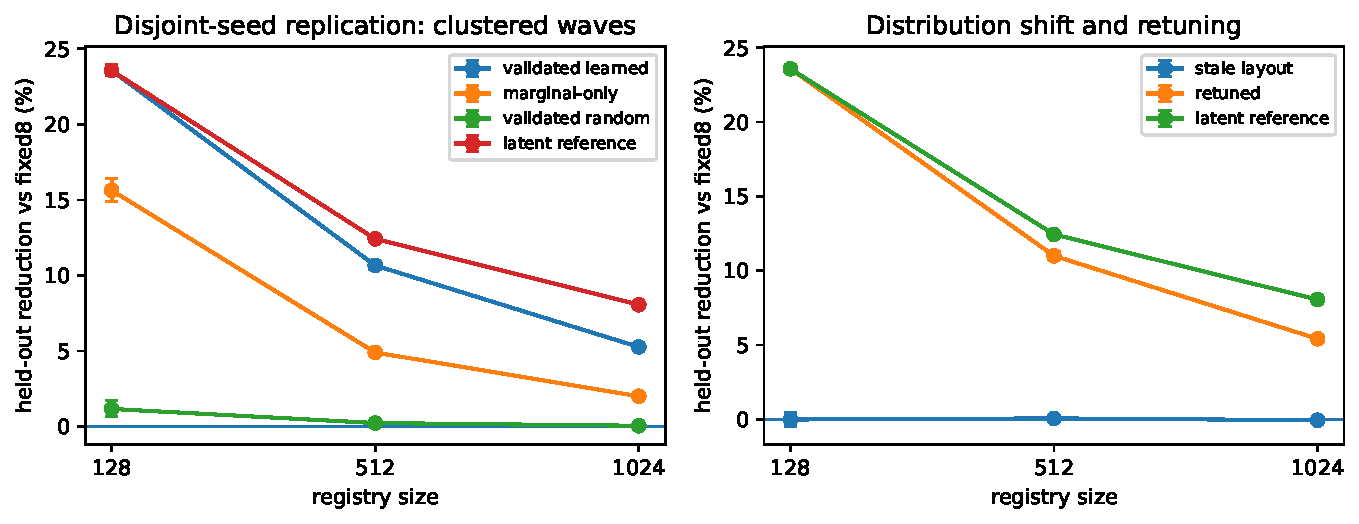
\includegraphics[width=.98\linewidth]{figures/v6_journal_extension.pdf}
\caption{Journal extension. Left: disjoint-seed clustered replication against marginal, validated-random, and latent-order references. Right: a latent cluster-permutation shift makes the old layout uninformative, while retuning on post-shift evidence recovers most of the structured benefit. Error bars are 95\% bootstrap intervals of the seed-level mean.}\label{fig:v6journal}
\end{figure}

The practical path invokes no tree DP. Median fitting time is approximately 0.02, 0.63, and 2.47 seconds at 128, 512, and 1,024 checks in this run. Fitting therefore remains control-plane work rather than an action-loop operation.

\subsection{RQ3: negative controls delimit the useful regime}
\begin{table}[H]\centering\small
\caption{Validated HACT on null controls. Changed counts validation decisions that selected the learned proposal; regress. counts held-out reductions below zero. Confidence intervals spanning zero are evidence against a systematic benefit, not evidence of equivalence.}\label{tab:v6nulls}
\begin{tabular}{@{}rlrrrr@{}}\toprule
Checks & Family & Mean (\%) & 95\% CI & Changed & Regress.\\\midrule
\csname @@input\endcsname generated_v6/nulls.tex
\bottomrule\end{tabular}
\end{table}

Global waves are analytically layout-insensitive under the balanced representation, and all sixty global replications yield exactly zero. Independent waves are more informative: means are -0.043\%, -0.010\%, and -0.013\%, with all three bootstrap intervals spanning zero. Validation often retains the incumbent, but it does not eliminate sampling error: the learned proposal is selected in 11/20, 6/20, and 9/20 seeds and produces 6, 3, and 6 small held-out regressions respectively. The unvalidated learned proposal regresses in 10/20, 9/20, and 10/20 independent seeds, so the hold-out guard avoids 4, 6, and 4 regressions without turning the selection procedure into a zero-regret guarantee.

This result sharpens the deployment rule: HACT needs stable higher-order locality, and validation is a risk-reduction device rather than proof that adaptation can never hurt.

\subsection{RQ4: distribution shift requires retuning}
The shift study uses twenty additional, disjoint seeds at each size. Training/validation regime A and post-shift regime B use independent latent permutations of the same clustered generator. The stale policy is chosen using only regime-A validation; the retuned policy is refit and selected only on regime-B training/validation, then both are evaluated on regime-B held-out data.

\begin{table}[H]\centering\small
\caption{Precommitted latent-permutation shift. Entries are mean reduction versus fixed8 with 95\% bootstrap intervals. The stale and retuned columns use the same validation/fallback rule in their respective regimes.}\label{tab:v6shift}
\begin{tabular}{@{}rccccc@{}}\toprule
Checks & Stale layout & Retuned & Latent ref. & Stale regress. & Retuned regress.\\\midrule
\csname @@input\endcsname generated_v6/shift.tex
\bottomrule\end{tabular}
\end{table}

A stale learned layout provides essentially no mean benefit after the latent permutation changes: -0.02\%, 0.05\%, and -0.07\% at 128, 512, and 1,024 checks. At 1,024 checks the bootstrap interval is entirely below zero (-0.10 to -0.03). Retuning restores 23.58\%, 10.99\%, and 5.41\% reductions, is positive in all sixty shifted replications, and shows no held-out regression. The retuning gains are 23.60, 10.94, and 5.47 percentage points; each size has a one-sided sign-test value of $9.54\times10^{-7}$. This validates the paper's decision to price migration and treat adaptation as a controlled process rather than a permanent learned ordering.

\subsection{RQ5: source-derived evidence supports, but does not duplicate, the synthetic result}
Two source studies answer different questions. First, a previously frozen confirmation cohort partitions archived cases into training, validation, and held-out confirmation sets for NetworkX~\cite{networkx}, Toolz~\cite{toolz}, and Future Code. That older study uses the research exact conditional compiler, not the v6 practical balanced compiler.

\begin{table}[H]\centering\small
\caption{Previously frozen source confirmation for the selected exact conditional layout versus original-order fixed8. Percentages are computed per held-out case from recorded source evidence.}\label{tab:sourceconfirm}
\begin{tabular}{@{}lrrrrr@{}}\toprule
Project & Checks & Cases & Mean (\%) & Median (\%) & Positive\\\midrule
NetworkX & 170 & 9 & 22.23 & 3.07 & 6/9\\
Toolz & 148 & 6 & 11.90 & 9.58 & 6/6\\
Future Code & 138 & 18 & 22.13 & 5.53 & 16/18\\
\midrule
All & -- & 33 & 20.30 & 5.73 & 28/33\\
\bottomrule\end{tabular}
\end{table}

Across 33 held-out source cases, 28 improve and five regress; the exact one-sided sign-test value for the 28/33 direction count is $3.31\times10^{-5}$. The per-case range is wide (-7.33\% to 63.56\%), showing that workload structure matters substantially. This cohort supports the existence of layout-sensitive structure in source-derived verification waves, while its different compiler and older data contract prevent us from presenting it as a replication of the practical v6 effect.

Second, the v5 codec replay re-aggregates twelve archived candidates under original fixed8, learned balanced8, and learned exact layouts. Learned balanced reduces whole-epoch compressed bytes by 41.84\% for NetworkX, 4.36\% for Toolz, and 18.53\% for Future Code. Across the twelve cases, batch-compressed application bytes are 416,046 for fixed8, 299,081 for learned balanced, and 278,831 for learned exact. Exhaustive diagnostic pages total 148, 95, and 87 respectively. Thus the practical layout retains real compression/page benefits while the exact reference quantifies additional headroom.

\subsection{RQ6: deployment economics remain service-specific}
The measured fixed-to-balanced compressed-byte difference is 116,965 bytes per twelve-candidate cohort. Under an explicitly assumed 64 KiB/s application goodput and $E=0$, Equation~\eqref{eq:latency} maps that byte difference to 1.784744 seconds of gross delivery time per cohort copy. This is arithmetic from measured application bytes, not a measured WAN speedup.

\begin{table}[H]\centering\small
\caption{Conditional minimum profitable copies of the same twelve-candidate cohort for whole-epoch compression, assuming $E=0$. Column headers are extra work per candidate; corresponding one-time cohort costs are 0.6, 6, and 60 seconds.}\label{tab:payback}
\begin{tabular}{@{}lrrr@{}}\toprule
Assumed goodput & 0.05 s & 0.5 s & 5 s\\\midrule
8 KiB/s & 1 & 1 & 5\\
64 KiB/s & 1 & 4 & 34\\
1 MiB/s & 6 & 54 & 538\\
\bottomrule\end{tabular}
\end{table}

The artifact stores 27 codec/rate/extra-cost scenarios and retains negative outcomes. A deployment should therefore decide that it needs hierarchical evidence first, measure the actual codec and bottleneck second, and only then decide whether a learned layout repays its fitting/migration work.

\subsection{Reproducibility, independent reconstruction, and failure provenance}
The journal extension stores 180 ordinary and sixty shift workload records, exact seed sets, layout orders, validation/held-out totals, dataset hashes, environment metadata, generated tables, and Figure~\ref{fig:v6journal}. An independent auditor regenerates each synthetic dataset, reconstructs compact-tree packet coverage without calling the producer's cost aggregation helper, recomputes every validation/held-out byte total, verifies the contract digest, and includes a deliberate tamper test. The final audit reports \texttt{PASS} for 180 ordinary and sixty shifted workloads and \texttt{PASS} for tamper detection.

The first audit attempt failed because the auditor incorrectly charged cold initialization once per cohort rather than once per epoch. No results were committed from that failed run. The accounting identity was corrected in the auditor only; the frozen contract, producer, seeds, baselines, and thresholds were unchanged. The rerun passed. Preserving this failure is useful evidence that the independent path was capable of rejecting a producer/auditor disagreement rather than merely echoing producer outputs.

\section{Implications and Threats to Validity}\label{sec:threats}
\paragraph{Operational implication.}
HACT should be selected only after the evidence service is selected. For a trusted final verdict, the root projection is the natural representation. For final per-check states, a flat ledger may be sufficient. When a system already requires bounded hierarchical diagnostics, learned-order balanced8 is the low-compilation-cost candidate, with the incumbent retained as a first-class fallback. Exact DP is a reference or optional offline candidate when additional byte savings justify compilation. The observed controls make this recommendation more specific, not weaker: layout learning has value only when the completion process presents exploitable structure.

\paragraph{Construct validity.}
The primary objective is serialized evidence cost under an explicit packet model. Padded bytes, canonical bytes, compressed bytes, pages, model tokens, and network latency are different quantities. We measure the first four where available and do not convert bytes to tokens by a heuristic ratio. The break-even model uses declared goodput and incremental work; sensitivity scenarios are planning inputs rather than measured latency. Whole-epoch compression also changes streaming semantics, so a smaller archive is not automatically a better online service.

\paragraph{Internal validity.}
Synthetic workloads use a frozen contract with disjoint train, validation, and held-out epochs; the source replay reuses fixed trusted records and execution order across layouts. Only three seeds occur in each synthetic cell, so the reported ranges are descriptive rather than high-precision population intervals. One interrupted synthetic run was resumed from 26 already-persisted records under the same frozen inputs. Independent reconstruction checks the stored arithmetic and serialization through a second code path, but it is not an external security audit.

\paragraph{External validity.}
The source evidence spans NetworkX, Toolz, and Future Code and consists of twelve archived candidates; it is not a new natural-bug corpus and does not measure model-generated repair quality. No hosted model is invoked in the v5 study. Physical-WAN trial count is zero, and the local TLS tests demonstrate protocol behavior rather than internet throughput, jitter, loss, or retransmission. Numerical BPE counts are also absent because the requested public tokenizer assets were unavailable in the recorded environment. Future evaluation should therefore prioritize paired remote delivery and live-agent runs where hierarchical diagnostics are actually consumed, rather than adding more synthetic byte-only variants.

\paragraph{Security and semantic boundary.}
Theorem~\ref{thm:safety} is conditional on a complete approved predicate set, correctly bound dependencies, a trusted checker, collision-resistant identity binding, and atomic local epoch/generation checks. HACT does not provide remote attestation, Byzantine consensus, non-repudiation, or an OS sandbox. A separate integration service must atomically bind the verified candidate to the integration head before merge or deployment. Evidence-layout independence protects the meaning of the declared contract; it cannot make an incomplete contract complete.

\section{Conclusion}\label{sec:conclusion}
Adaptive HACT turns hierarchical verification evidence into a representation-optimization problem under a semantic invariant. Stable identities and generation fencing separate acceptance from layout, while completion hyperedges provide the cost signal needed to exploit higher-order locality. The empirical result is deliberately conditional: all nine clustered synthetic seeds improve, independent/global controls do not, and source replays show 4.36--41.84\% whole-epoch compressed savings for the practical learned-balanced layout while the exact reference quantifies remaining headroom. Semantic outputs remain invariant across the replayed layouts. These results support HACT where hierarchical evidence delivery is a real systems cost; they do not imply a universal agent, token, or WAN speedup. That separation between semantic safety, representation efficiency, and deployment economics is the paper's main systems contribution.

\begin{thebibliography}{30}
\sloppy
\bibitem{rothermel} Gregg Rothermel, Roland H. Untch, Chengyun Chu, and Mary Jean Harrold.
\newblock Prioritizing test cases for regression testing.
\newblock \emph{IEEE Transactions on Software Engineering}, 27(10):929--948, 2001.
\newblock \url{https://doi.org/10.1109/32.962562}.

\bibitem{ekstazi} Milos Gligoric, Lamyaa Eloussi, and Darko Marinov.
\newblock Practical regression test selection with dynamic file dependencies.
\newblock \emph{Proceedings of ISSTA}, 2015.
\newblock \url{https://users.ece.utexas.edu/~gligoric/papers/GligoricETAL15Ekstazi.pdf}.

\bibitem{namerts} You Wang, Michael Pradel, and Zhongxin Liu.
\newblock Names Are All You Need: Effective and Safe Regression Test Selection for Python.
\newblock arXiv:2605.25356v1, May 2026.
\newblock \url{https://arxiv.org/abs/2605.25356v1}.

\bibitem{acar} Umut Acar, Guy Blelloch, Matthias Blume, Robert Harper, and Kanat Tangwongsan.
\newblock A Library for Self-Adjusting Computation.
\newblock \emph{Electronic Notes in Theoretical Computer Science}, 148:127--154, 2006.
\newblock \url{https://doi.org/10.1016/j.entcs.2005.11.043}.

\bibitem{build} Andrey Mokhov, Neil Mitchell, and Simon Peyton Jones.
\newblock Build Systems \`a la Carte.
\newblock \emph{Proceedings of the ACM on Programming Languages}, 2(ICFP), Article 79, 2018.
\newblock \url{https://doi.org/10.1145/3236774}.

\bibitem{alphabetic} Hirendu Vaishnav and Massoud Pedram.
\newblock Alphabetic Trees: Enumeration and Optimization with Applications to VLSI Design.
\newblock Author-hosted manuscript, Sections 4.1--4.4; date not established from the retrieved manuscript.
\newblock \url{https://www.mpedram.com/Papers/alp-trees-journal.pdf}.

\bibitem{hmt} Ziheng Shangguan, Aviv Yaish, and Dahlia Malkhi.
\newblock Authenticated Data Structures for Dynamic Workloads.
\newblock arXiv:2608.25206v1, August 2026.
\newblock \url{https://arxiv.org/abs/2608.25206v1}.

\bibitem{pcaa} Zexun Wang.
\newblock Proof-Carrying Agent Actions: Model-Agnostic Runtime Governance for Heterogeneous Agent Systems.
\newblock arXiv:2606.04104v1, June 2026.
\newblock \url{https://arxiv.org/abs/2606.04104v1}.

\bibitem{vpcontrol} Zihao Zheng, Baichuan Li, Junyi Yao, and Jiayu Long.
\newblock Engineering Reliable Commit Gates for Agentic AI: Cost-Aware Verification Portfolios under Common-Mode Data Failures.
\newblock arXiv:2609.10969v1, September 2026.
\newblock \url{https://arxiv.org/abs/2609.10969v1}.

\bibitem{hoeffding} Wassily Hoeffding.
\newblock Probability Inequalities for Sums of Bounded Random Variables.
\newblock \emph{Journal of the American Statistical Association}, 58(301):13--30, 1963.
\newblock \url{https://doi.org/10.1080/01621459.1963.10500830}.

\bibitem{networkx} NetworkX developers.
\newblock NetworkX 3.6.1 release documentation and distributed source tests.
\newblock \url{https://networkx.org/documentation/stable/release/release_3.6.1.html}.

\bibitem{toolz} PyToolz contributors.
\newblock Toolz API documentation and distributed source tests.
\newblock \url{https://toolz.readthedocs.io/en/stable/api.html}.

\bibitem{atkins} Jonathan E. Atkins, Erik G. Boman, and Bruce Hendrickson.
\newblock A Spectral Algorithm for Seriation and the Consecutive Ones Problem.
\newblock \emph{SIAM Journal on Computing}, 28(1):297--310, 1998.
\newblock \url{https://doi.org/10.1137/S0097539795285771}.

\bibitem{herbster} Mark Herbster and Manfred K. Warmuth.
\newblock Tracking the Best Expert.
\newblock \emph{Machine Learning}, 32:151--178, 1998.
\newblock \url{https://doi.org/10.1023/A:1007424614876}.

\bibitem{geulen} Sascha Geulen, Berthold V\"ocking, and Melanie Winkler.
\newblock Regret Minimization for Online Buffering Problems Using the Weighted Majority Algorithm.
\newblock \emph{Proceedings of COLT}, pages 132--143, 2010.
\newblock \url{https://www.learningtheory.org/colt2010/conference-website/papers/105geulen.pdf}.

\bibitem{cesa} Nicol\`o Cesa-Bianchi, Ofer Dekel, and Ohad Shamir.
\newblock Online Learning with Switching Costs and Other Adaptive Adversaries.
\newblock \emph{Advances in Neural Information Processing Systems}, 26, 2013.
\newblock \url{https://papers.neurips.cc/paper/5151-online-learning-with-switching-costs-and-other-adaptive-adversaries.pdf}.

\bibitem{swebench} Carlos E. Jimenez, John Yang, Alexander Wettig, Shunyu Yao, Kexin Pei, Ofir Press, and Karthik Narasimhan.
\newblock SWE-bench: Can Language Models Resolve Real-World GitHub Issues?
\newblock \emph{International Conference on Learning Representations}, 2024.
\newblock \url{https://arxiv.org/abs/2310.06770}.

\bibitem{otel} OpenTelemetry contributors.
\newblock Batch Processor documentation, official collector implementation.
\newblock Accessed September 20, 2026.
\newblock \url{https://github.com/open-telemetry/opentelemetry-collector/tree/main/processor/batchprocessor}.
\bibitem{tiktoken} OpenAI contributors.
\newblock tiktoken: BPE tokenization implementation and encoding registry.
\newblock Accessed September 21, 2026; package/vocabulary unavailable in the v5 measurement runtime.
\newblock \url{https://github.com/openai/tiktoken}.
\bibitem{sweharness} SWE-bench contributors.
\newblock The Harness: Docker-based patch evaluation reference.
\newblock Accessed September 20, 2026.
\newblock \url{https://www.swebench.com/SWE-bench/reference/harness/}.
\bibitem{rfc6349} B. Constantine, G. Forget, R. Geib, and R. Schrage.
\newblock Framework for TCP Throughput Testing. RFC 6349, August 2011.
\newblock \url{https://www.rfc-editor.org/rfc/rfc6349.html}.

\bibitem{sweagent} John Yang, Carlos E. Jimenez, Alexander Wettig, Kilian Lieret, Shunyu Yao, Karthik Narasimhan, and Ofir Press.
\newblock SWE-agent: Agent-Computer Interfaces Enable Automated Software Engineering.
\newblock arXiv:2405.15793, 2024.
\newblock \url{https://arxiv.org/abs/2405.15793}.

\bibitem{agentless} Chunqiu Steven Xia, Yinlin Deng, Soren Dunn, and Lingming Zhang.
\newblock Agentless: Demystifying LLM-based Software Engineering Agents.
\newblock arXiv:2407.01489, 2024.
\newblock \url{https://arxiv.org/abs/2407.01489}.

\bibitem{openhands} Xingyao Wang et al.
\newblock OpenHands: An Open Platform for AI Software Developers as Generalist Agents.
\newblock arXiv:2407.16741, 2024.
\newblock \url{https://arxiv.org/abs/2407.16741}.

\bibitem{sweevo} Tue Le, Minh V. T. Thai, Dung Nguyen Manh, Huy Phan Nhat, and Nghi D. Q. Bui.
\newblock SWE-EVO: Benchmarking Coding Agents in Long-Horizon Software Evolution Scenarios.
\newblock arXiv:2512.18470, revised 2026.
\newblock \url{https://arxiv.org/abs/2512.18470}.

\bibitem{verificationdriven} Qinghua Lu et al.
\newblock Verification-Driven AI Engineering: A Software Engineering Discipline for Agentic AI Systems.
\newblock SSRN 6430979, 2026.
\newblock \url{https://doi.org/10.2139/ssrn.6430979}.

\bibitem{aiware} Qinghua Lu et al.
\newblock Engineering Agentic Systems: Toward Verification-First AIware Engineering.
\newblock \emph{IEEE Software}, 43(5):22--29, 2026.
\newblock \url{https://doi.org/10.1109/MS.2026.3697911}.

\bibitem{traceassurance} George Paduraru, Cristian Bouruc, and Alin Stefanescu.
\newblock A Trace-Based Assurance Framework for Agentic AI Orchestration.
\newblock \emph{Proceedings of ENASE}, pages 420--427, 2026.
\newblock \url{https://doi.org/10.5220/0014840300004015}.

\end{thebibliography}

\appendix
\section{Optional Fixed-Share Analysis: Not the Deployment Recommendation}\label{app:tracking}
This section retains v3's former Theorem 4 and its assumptions. It is an optional comparator, not the practical selector recommended in v4. On the measured streams it loses to the deterministic priced-window rule in three regimes. We have not searched for a favorable adversarial stream after seeing those results, and make no claim that a tracking bound implies an empirical advantage.
\subsection{Fixed-share weights with maximal coupling}
Let a declared bound $R$ cover each round's loss spread, $\max_i\ell_t(i)-\min_i\ell_t(i)\le R$. Reject a measurement exceeding it instead of clipping the cost. Define $z_{t,i}=(\ell_t(i)-\min_j\ell_t(j))/R$. Starting at $p_1(i)=1/K$, update
\begin{align}
 q_{t+1}(i)&=\frac{p_t(i)\exp(-\eta z_{t,i})}{\sum_jp_t(j)\exp(-\eta z_{t,j})},\\
 p_{t+1}(i)&=(1-\alpha)q_{t+1}(i)+\alpha/K,\quad 0<\eta\le1,\;0\le\alpha<1.\label{eq:share}
\end{align}
Independent draws from each new distribution can waste migrations. Instead, conditional on $A_t=i$, retain $i$ with probability $\min\{1,p_{t+1}(i)/p_t(i)\}$. If it is not retained, sample from the normalized positive residual $(p_{t+1}-p_t)_+$. This maximal coupling has marginal $p_{t+1}$ and switch probability $\operatorname{TV}(p_t,p_{t+1})$. Established dependent-sampling methods motivate this choice~\cite{geulen}; we do not claim it as a new sampling algorithm.

\begin{theorem}[Catalogue tracking with migration]\label{thm:tracking}
Assume a frozen catalogue, a fixed exogenous sequence of full-information loss vectors, spread at most $R$, and $M_{ij}\le M$. For any comparator path $u_{1:T}$ with $s$ changes and $0<\alpha<1$, the coupled policy satisfies
\begin{align}
 \E[\mathcal L_T]-\sum_t\ell_t(u_t)
 \le{}& R\left[\frac{\log K+s\log(K/\alpha)+(T-1-s)\log(1/(1-\alpha))}{\eta}
             +\frac{\eta T}{8}\right]\nonumber\\
 &+M(T-1)(\eta+\alpha).\label{eq:tracking}
\end{align}
For $\alpha=0$ the stationary-comparator bound has numerator $\log K$ and applies only to $s=0$.
\end{theorem}
\begin{proof}
The fixed-share update is exponential weighting over paths with an initial uniform prior, self-transition mass at least $1-\alpha$, and transition mass at least $\alpha/K$. The negative log prior of a path with $s$ switches is bounded by the numerator. The bounded exponential-moment inequality gives expected normalized service regret at most that numerator divided by $\eta$, plus $\eta T/8$ (Appendix~\ref{app:online}). Since losses are exogenous, the weights are independent of the sampled action path, and the coupling preserves each unconditional marginal. Exponential reweighting changes total variation by at most $\eta$; uniform mixing adds at most $\alpha$. Thus the expected switch count is at most $(T-1)(\eta+\alpha)$. Multiplication by $M$ and addition of service regret proves the bound.\end{proof}
The bound also upper-bounds regret relative to the comparator's service \emph{plus} nonnegative migration cost, but can be quite loose. It is not a per-run improvement guarantee. Choosing fixed $\eta=.5$ and $\alpha=.01$, as in our frozen experiment, need not make this bound sublinear with increasing $T$. Horizon-dependent tuning yields sublinear stationary bounds (Appendix~\ref{app:online}), without creating a guarantee against arbitrary reactive agents or newly introduced catalogue entries.


\section{Block-Backbone Compiler: Retained Ablation}\label{sec:block}
The exact compiler's cubic cost makes frequent full recompilation inappropriate. For a supplied display order, divide the leaves into consecutive blocks of at most $s$ leaves, and fix a compact $b$-ary macro-tree on those blocks. Optimize each block's microtree using its restricted completion waves and strict-epoch initialization cost. Replace each macro leaf by its optimized microtree. No evaluation waves enter this process.

\begin{proposition}[Exactness in the block-backbone class]\label{prop:block}
With display order, block boundaries and macro-tree fixed, independent exact optimization of the blocks minimizes the training objective over every layout in that restricted class. The dynamic-programming work is $O(bns^2)$ with $O(bs^2)$ reusable DP workspace, excluding order learning and wave preparation.
\end{proposition}
\begin{proof}
Every macro node covers a fixed union of complete blocks, so its activation weight and packet price are constant across the class. All variable costs lie inside disjoint microtrees. The objective is a constant plus the sum of their independent objectives. Conditional exactness therefore gives the minimizing member. There are at most $\lceil n/s\rceil$ subproblems, each of size at most $s$, yielding the stated DP bound. Reusing the subproblem arrays yields the workspace bound.\end{proof}
For the reference implementation, $M$ recorded waves and $L$ total wave memberships add filtering and weight-preparation work of $O(\lceil n/s\rceil L+Mns)$, and storage for the input, output and local $M\times s$ arrays. This is not a linear-time claim for the entire pipeline. Dense affinity construction and order learning remain separate costs. No bounded approximation ratio against the unrestricted exact tree is asserted; held-out cost can deteriorate. The historical experiment froze $s=32$ before measurement. Its negative result motivates excluding this compiler from the v5 practical path.


The original 18-workload v4 scaling data remain in the artifact. Block DP reduced fitting time relative to exact DP but lost to same-order balanced fixed8 in held-out bytes. Restricted-class exactness is a mathematical property, not an empirical recommendation.

\section{Information Separations Retained from Earlier Versions}\label{app:separations}
These results concern the information available to a selector. They are not hardness results for all adaptive tree algorithms, and they do not imply that a complete hypergraph must be recovered: interval hit statistics are sufficient for a fixed order and objective.

\subsection{Marginals do not determine a co-invalidation optimum}
Consider four ordered leaves, binary trees, and a constant internal packet price $c>0$. Let $\mathcal D_A$ choose $\{0,1\}$ or $\{2,3\}$ equiprobably and $\mathcal D_B$ choose $\{0,3\}$ or $\{1,2\}$ equiprobably. All leaf marginal activation probabilities equal $1/2$ in both distributions. The root and every three-leaf interval are always activated. The five tree shapes therefore fall into the following classes:
\begin{center}\small
\begin{tabular}{@{}lrr@{}}\toprule
Ordered tree & $J_A/c$ & $J_B/c$\\\midrule
$((0,1),(2,3))$ & 2 & 3\\
$(0,((1,2),3))$, $((0,(1,2)),3)$ & 3 & 2.5\\
$(0,(1,(2,3)))$, $(((0,1),2),3)$ & 2.5 & 3\\\bottomrule
\end{tabular}
\end{center}
Optimal costs are $2c$ and $2.5c$. A deterministic marginal-only selector receives identical input and must choose the same class, incurring at least $c/2$ regret on one distribution. The last class is weakly dominated by the balanced tree. If a randomized selector chooses the balanced tree with probability $q$, its regrets are at least $(1-q)c$ and $qc/2$. Their maximum is minimized at $q=2/3$ and equals $c/3$, which is attainable for this instance. A fixed initialization price adds the same $3c$ to all binary shapes and does not alter the separation.

\subsection{Joint invalidation does not determine progressive layout}
Every epoch now invalidates all four checks, and execution order is $(0,1,2,3)$ with singleton completion waves. In workload $A$, check 0 fails, so only its wave is executed. In workload $B$, check 3 fails, so all four checks execute. Initial invalidation is identical, even jointly.

Every binary tree has three internal nodes. Its cost in $A$ is $(3+\operatorname{depth}(0))c$, minimized at $4c$ by a root-0 comb. Its cost in $B$ is $(3+\sum_i\operatorname{depth}(i))c$, minimized at $11c$ by the balanced tree. The root-0 comb costs $12c$ in $B$, whereas the balanced tree costs $5c$ in $A$. The remaining shapes are weakly dominated. An invalidation-only randomized selector using a root-0 comb with probability $p$ incurs regrets at least $(1-p)c$ and $pc$, whose maximum is at least $c/2$. A deterministic selector incurs at least $c$. The example proves a separation between stale-set information and schedule-induced completion information; it does not prohibit a selector that observes both.

\section{Cost, Statistical, and Online Proof Details}\label{app:online}
\subsection{Exact serialization accounting}
On the first refresh in a strict epoch, every internal node emits one packet. Within a fixed tree and registry, the cache uses monotone descendant-generation stamps. A subsequent wave emits a node's packet exactly when at least one final record in its semantic coverage changed. Multiple completed descendants in one wave still induce one packet at that node. Summing initialization and wave contributions yields Equation~\eqref{eq:strict}. After migration, a new kernel remaps canonical IDs and the old ordinal cache is not reused; the entire cold rebuild is charged in Equation~\eqref{eq:migration}.

This argument concerns logical and actual serialized packet lengths. The separate v4 study measures controlled application-level export time, not production-network throughput. It does not include raw log streams, TLS framing, operating-system scheduling, or Python traversal costs. The reference kernel validates and traverses trees and is not claimed to have logarithmic total runtime. Small contexts do not imply small total system state.

\subsection{Full-refresh lower bound and global negative control}
For an $n$-leaf tree with $m$ internal nodes, the number of edges is $n+m-1$, so $\sum_vd_v=n+m-1$. Therefore
\begin{equation}
 W(L)=S(n-1)+(H+S)m\ge S(n-1)+(H+S)\left\lceil\frac{n-1}{b-1}\right\rceil.
\end{equation}
The inequality follows from $n-1=\sum_v(d_v-1)\le m(b-1)$. At $n=64,b=8$, a complete eight-child construction attains the bound with $m=9$ and $W=27,648$ bytes. Thus all selected global-control layouts can tie an analytically minimal full refresh. Strict initialization followed by one global completion wave costs $2W$. This explains the exact negative control without assuming every balanced tree at every $n$ attains the lower bound.

\subsection{Uniform statistical control at a fixed order}
For one activation wave per episode and a fixed registry order, let $M_n=n(n+1)/2$ and
\[
 \epsilon=\sqrt{\log(2M_n/\delta)/(2m)}.
\]
The interval hit indicators are bounded independent variables \emph{across} independent episodes, though checks within an episode may be arbitrarily dependent. Hoeffding plus a union bound gives simultaneous interval-frequency error at most $\epsilon$. For every feasible tree, $|\widehat J(T)-J(T)|\le W(T)\epsilon$. Inserting the empirical minimizer gives regret at most $[W(\widehat T)+W(T^*)]\epsilon\le2(n-1)C\epsilon$. This is the original HACT bound, retained for attribution. It is not automatically valid uniformly over arbitrary data-selected permutations; the separate held-out catalogue bound in Proposition~\ref{prop:validation} addresses that selection step.

For strict epochs with at most $q$ completion waves, a loose range is $B=(q+1)(n-1)C$. Under the evaluated sequential eight-record flush rule with at most one final record per obligation, $q\le\lceil n/8\rceil$. A narrower observed range is not automatically a proved bound for an unobserved deployment distribution.

\subsection{Maximal coupling and its switch count}
Let $p,p'$ be consecutive distributions. The probability mass that remains at index $i$ under the coupling is $\min(p_i,p'_i)$. The remaining mass is distributed as $(p'-p)_+$, so the new marginal is exactly $p'$ and
\[
 \Prb(A_{t+1}\ne A_t)=1-\sum_i\min(p_i,p'_i)=\operatorname{TV}(p,p').
\]
For exponential reweighting by $a_i=\exp(-\eta z_i)$ with $z_i\in[0,1]$, the normalizer is at most one, hence $q_i\ge e^{-\eta}p_i$. Thus $\sum_i\min(p_i,q_i)\ge e^{-\eta}$ and $\operatorname{TV}(p,q)\le1-e^{-\eta}\le\eta$. Mixing $q$ with the uniform distribution by weight $\alpha$ changes total variation by at most $\alpha$. The triangle inequality gives the switch bound in Theorem~\ref{thm:tracking}. Zero old mass is never the probability of a selected previous action in exact arithmetic; the implementation rejects inconsistent checkpoints.

\subsection{Fixed-share path argument}
A path $u_{1:T}$ with $s$ changes has prior mass at least
\[
 P(u_{1:T})\ge K^{-1}(\alpha/K)^s(1-\alpha)^{T-1-s}.
\]
The share update is the forward recursion for exponential weighting over such paths. If $Z_t=\sum_ip_t(i)\exp(-\eta z_{t,i})$, then the bounded exponential-moment inequality implies
\[
 \log Z_t\le-\eta\langle p_t,z_t\rangle+\eta^2/8.
\]
On the other hand, the cumulative mixture likelihood is at least the comparator path's prior times its exponential loss. Combining the inequalities yields
\[
 \sum_t\langle p_t,z_t\rangle-\sum_tz_{t,u_t}
 \le-\log P(u_{1:T})/\eta+\eta T/8.
\]
Centering losses by their per-round minimum cancels in regret, and multiplying by $R$ restores byte units. For a fixed exogenous cost sequence, each $p_t$ is determined by past full-information observations independently of the sampled action sequence; maximal coupling preserves its marginal. Therefore expected sampled service equals the left-side weighted service. Adding at most $M$ per expected switch proves Equation~\eqref{eq:tracking}.

The result does not cover a cost sequence chosen in reaction to the coupled hidden action history. It also does not cover agents changing future task choices because a layout changed the text they read. These limitations are why the paper distinguishes a verification-plane cost experiment from an end-to-end learning claim.

\subsection{Horizon dependence and break-even interpretation}
For $K\ge2$, $s=0$, and $\alpha=0$, write $B_T=RT/8+M(T-1)$. The bound is $R\log K/\eta+\eta B_T$. When $\sqrt{R\log K/B_T}\le1$, choosing that learning rate gives at most $2\sqrt{R\log K\,B_T}$ expected regret, which is sublinear for fixed $R,M,K$. This is an established style of switching-cost bound, not a new rate. With a known sparse switch budget, selecting a horizon-dependent share similarly prices tracking complexity. Our fixed-parameter experiments do not invoke such a tuned asymptotic guarantee.

A single empirical switch with estimated future saving $d$ and anticipated remaining horizon $h$ satisfies the familiar break-even inequality $hd>M_{ij}$. This is arithmetic, not a drift theorem: savings may reverse before $h$ events. The included window rule uses its past 64 events as that estimate and is deliberately reported as a heuristic. All choices, including greedy choices that ignore migration when deciding, are charged their actual transition price during evaluation.

\section{Experimental Reproduction and Threats to Validity}
\subsection{Software and data identities}
The archived v3 runs used Python 3.13.5 on Linux x86\_64; exact installed package and platform records accompany emitted reports. Compilers were measured with \texttt{OPENBLAS\_NUM\_THREADS=1}. No accelerator is required. Vendored upstream sources and tests are retained with their notices. Every fresh mutation is checked against its archived base-source hash, replacement span, and resulting source hash. This binds a result to a specific intervention, not a natural historical bug distribution.

For the archived v3 record, there are three named output categories: \texttt{historical/results\_v2} contains previous observations; \texttt{results/v3} contains v3's generated layouts, raw waves, online paths, fresh subprocess reports, and harness records; \texttt{paper/generated} contains tables regenerated from those files. Running reproduction in a fresh destination avoids overwriting the released record. The release manifest identifies the exact packaged files. The final extracted archive is tested again before delivery. New v4 transfers, compiler traces, contexts, summaries and audits are stored separately in \texttt{results/v4}; they do not change the number of earlier checker or harness executions. V5 adds \texttt{results/v5} for the practical catalogue, archived-source re-aggregation, conditional deployment accounting and failed BPE attempts. Neither a new layout nor a reproduced experiment is counted as another repaired candidate.

\subsection{Costs not hidden by replay}
Ordering measurements include strict initialization; online traces explicitly use persistent-state incremental service plus cold switch prices. These are different lifecycles. Source replay uses a fixed previous ranker; fresh paired executions hold that ranker constant. The I/O harness does not compare different model-generated solutions: it sends identical scripted patch content to the same real runtime under different gates. Its model endpoint produces no provider token-usage field, so absent usage remains null in the records. Prompt byte lengths are measured directly and never converted to tokens by a heuristic multiplier.

Timing rows report outer-wrapper or active-episode boundaries explicitly. The wrapper's internal total ends just before final report and packet-file writes; the fresh study additionally records the outer call duration including those writes. Fit, contract approval, and baseline preparation are setup costs, not silently amortized into a claimed end-to-end speedup. With only three harness repeats, ranges are more honest than a precise broad-population confidence claim.

\subsection{Test adequacy, nondeterminism, and I/O}
The fixture performs real disk and loopback I/O but is intentionally controlled. It is not a test of internet reliability, production SQLite contention, nondeterministic service responses, or all flaky-test policies. When a collected check is skipped, missing, or inconsistent, it is not accepted as a pass. Two contradictory final records in one epoch trigger conflict handling, and an operator must establish a new epoch rather than cherry-pick the favorable record. Actual source tests can themselves be incomplete; agreement with their oracle is only agreement with the declared acceptance contract.

\section{Artifact Usage and Integration Contract}
A reviewed operator baseline is initialized outside candidate write scopes:
\begin{verbatim}
python -m ichact init --project /work/trusted-baseline \
  --contract /work/contracts/approved.json \
  --output /work/reports/baseline --test-path tests

python -m ichact verify --project /work/candidate \
  --contract /work/contracts/approved.json \
  --output /work/reports/candidate-001 \
  --layout /work/contracts/layout.json
\end{verbatim}
A layout must match the full semantic registry. The optional execution-order file is separate and must also be an exact permutation, never a subset. Legacy schema-1 contracts must be reviewed and reinitialized; the software does not silently reinterpret them.

The Future Code gate invokes the installed module or a pinned absolute bridge path outside the candidate:
\begin{verbatim}
python -m ichact.future_bridge \
  --contract /work/contracts/approved.json \
  --reports /work/verification-reports \
  --layout /work/contracts/layout.json
\end{verbatim}
The working directory is the candidate snapshot. Exit 0 means complete current pass; nonzero means rejection or unknown. This CLI does not itself deploy or merge. The original harness performs its own staged-source fingerprint and integration checks. For hostile code, use an outer container/VM and do not give it access to secrets or trusted contract storage.

The artifact contains an actual scripted harness campaign, a separate live-endpoint configuration guide, deterministic tests, an independent audit, and an isolated reproduction launcher. The live guide is a deployment recipe, not evidence that paid inference or hosted evaluation was performed.

\end{document}
